\documentclass[12pt]{article}

% --- Page geometry ---
\usepackage[margin=1in]{geometry}

% --- Math and symbols ---
\usepackage{amsmath,amssymb,amsthm}
\usepackage{mathtools}

% --- Figures and tables ---
\usepackage{graphicx}
\usepackage{booktabs}
\usepackage{multirow}
\usepackage{array}

% --- Typography ---
\usepackage{microtype}
\usepackage{natbib}
\usepackage{hyperref}
\usepackage[capitalize]{cleveref}
\usepackage{algorithm}
\usepackage{algpseudocode}

% --- Line numbers for review ---
\usepackage{lineno}
\linenumbers  % For review submission

% --- Theorem environments ---
\newtheorem{proposition}{Proposition}
\newtheorem{definition}{Definition}
\newtheorem{remark}{Remark}
\newtheorem{corollary}{Corollary}

% --- Custom commands ---
\newcommand{\Tsys}{T_{\mathrm{sys}}}
\newcommand{\fsys}{f_{\mathrm{sys}}}
\newcommand{\Fsys}{F_{\mathrm{sys}}}
\newcommand{\Ssys}{S_{\mathrm{sys}}}
\newcommand{\MAE}{\mathrm{MAE}}
\newcommand{\IE}{\mathrm{IE}}
\newcommand{\btheta}{\boldsymbol{\theta}}
\newcommand{\blambda}{\boldsymbol{\lambda}}
\newcommand{\bx}{\mathbf{x}}
\newcommand{\given}{\,|\,}

% --- Title ---
\title{A Binary Threshold for Component Identification\\
  in $k$-out-of-$m$ Systems}

\author{
  Alexander Towell\thanks{
    Department of Computer Science,
    Southern Illinois University Edwardsville, Edwardsville, IL 62026, USA.
    Email: \href{mailto:lex@metafunctor.com}{\texttt{lex@metafunctor.com}}.
    ORCID: 0000-0001-6443-9897.}
}

\date{}

\begin{document}

\maketitle

% ===========================================================================
% ABSTRACT
% ===========================================================================

\begin{abstract}
Estimating individual component lifetime parameters from $k$-out-of-$m$ system
failure data is a fundamental problem in reliability engineering.  We show that
the system density $\fsys(t; \blambda)$ is invariant under permutation of
component parameters, creating $m!$ equivalent modes on the likelihood surface.
This symmetry renders individual parameters non-identifiable from system-level
data alone, and domain knowledge (ordering constraints, heterogeneous fleet
structures) provides negligible improvement (${\approx}1\times$).
We demonstrate empirically that a \emph{binary identification threshold} governs this problem:
any single component-level observation breaks the symmetry, while no amount of
system-level data can.  We develop three observation mechanisms with explicit
likelihoods for general $k$-out-of-$m$ systems: periodic inspection,
generalized masking, and partial autopsy.  A Monte Carlo comparison
($m = 4$ exponential components, $n = 300$ observations, $R = 50$--$100$ replicates)
yields two central findings.  First, inspecting just one of $m = 4$ components
after failure captures 87\% of the improvement from inspecting all four
($\MAE$: $0.200 \to 0.062$ at $r = 1$, vs.\ $0.042$ at $r = m$).
Second, temporal resolution is irrelevant: inspection intervals from
$\delta = 0.1$ to $\delta = 2.0$ produce identical accuracy
($\MAE \approx 0.032$).  The symmetry-breaking information is the
\emph{identity} of a component (which one failed or survived), not the
\emph{timing} of its failure.  All methods are implemented in the open-source
R package \texttt{kofn}.
\end{abstract}

\medskip
\noindent
\textbf{Keywords:}
$k$-out-of-$m$ systems; permutation symmetry; component estimation;
masked failure data; periodic inspection; maximum likelihood estimation;
reliability

% ===========================================================================
% 1. INTRODUCTION
% ===========================================================================

\section{Introduction}\label{sec:intro}

Consider a redundant power supply with four independent modules in a parallel
configuration: the system operates as long as at least one module functions.
An engineer observes system failure times for a fleet of 300 such units and
seeks to estimate the individual module failure rates.  The system-level
data are abundant, yet the parameter estimates are unreliable---not because
of sample size, but because the system density is invariant under any
permutation of the module labels.  Swapping the roles of the fastest and
slowest modules yields exactly the same likelihood.

This \emph{permutation symmetry} is not merely a computational nuisance; it
is a structural barrier to identifiability.  The likelihood surface exhibits
$m!$ equivalent modes, and the maximum likelihood estimator (MLE) converges
to the symmetric point where all rates appear equal, regardless of the true
heterogeneity.  For the parallel power supply ($k = m = 4$), there are $24$
equivalent modes.  Even for a 2-out-of-4 system, the density retains full
permutation symmetry, and the $24$ modes persist.

The standard framing of component estimation from system data treats the
problem as one of censoring: at system failure time $\Tsys$, some component
lifetimes are observed (or bounded) and others are censored
\citep{BarlowProschan1975, LawlessBook2003}.
Recent work by \citet{QiangPena2025} combines component and system test
data via shrinkage estimation, but assumes at least some component-level
observations are already available.  For series systems ($k=1$),
this is the classical masked cause-of-failure problem, where the critical
component's identity is latent \citep{Miyakawa1984, LinUsherGuess1993,
Usher1996, KunduBasu2000}.  For
general $k$-out-of-$m$ systems, the censoring structure is richer---$k-1$
components are left-censored, one is exact, and $m-k$ are
right-censored---but the symmetry barrier persists at every $k$.

This paper makes three contributions.
%
First, we reframe $k$-out-of-$m$ component estimation as a
\emph{symmetry-breaking problem} rather than merely a censoring problem.
We prove that the system density of any $k$-out-of-$m$ system is invariant
under permutation of component parameters (\cref{prop:symmetry}), formally
establishing that system-level data alone cannot identify individual
parameters at any $k$.
%
Second, we develop three component-level observation mechanisms with explicit
likelihoods for general $k$-out-of-$m$ systems:
\emph{periodic inspection} (\cref{sec:periodic}), which interval-censors
each component's failure time;
\emph{generalized masking} (\cref{sec:masking}), which extends the masked
cause-of-failure framework from series to arbitrary $k$; and
\emph{partial autopsy} (\cref{sec:autopsy}), which reveals the binary
failed/survived status of a subset of components.
%
Third, we conduct a systematic Monte Carlo comparison of six
symmetry-breaking mechanisms, with sensitivity analyses for masking noise,
inspection granularity, and autopsy coverage (\cref{sec:monte-carlo}).
The comparison reveals a binary identification threshold:
\begin{enumerate}
  \item \textbf{Phase transition at $r=1$.}  Inspecting a single component
    after system failure captures 87\% of the improvement from full autopsy.
    The transition is from $\MAE = 0.200$ (system-only) to $\MAE = 0.062$
    (one component inspected), vs.\ $0.042$ at $r = m$.  The first
    component observation collapses the $m!$ modes; additional observations
    refine, but the identification is already achieved.
  \item \textbf{Temporal resolution is irrelevant.}  Periodic inspection at
    intervals of $\delta = 0.1$ versus $\delta = 2.0$ (a $20\times$ range
    in granularity) produces identical estimation accuracy
    ($\MAE \approx 0.032$).  The symmetry-breaking information is the
    \emph{identity} of a component (which one failed or survived), not
    the precision of when.
\end{enumerate}

The paper is organized as follows.  \Cref{sec:background} establishes the
mathematical framework for coherent systems, censoring structures, and the
likelihood.  \Cref{sec:symmetry} formalizes the permutation symmetry barrier
and introduces a taxonomy of symmetry-breaking mechanisms.
\Cref{sec:mechanisms} develops the three component-level mechanisms with
their likelihoods.  \Cref{sec:monte-carlo} presents the Monte Carlo
comparison.  \Cref{sec:discussion} provides practical recommendations.
\Cref{sec:software} describes the \texttt{kofn} R package.
\Cref{sec:conclusion} concludes.

% ===========================================================================
% 2. BACKGROUND AND NOTATION
% ===========================================================================

\section{Background and Notation}\label{sec:background}

\subsection{Coherent systems and \texorpdfstring{$k$-out-of-$m$}{k-out-of-m} structure}
\label{sec:coherent}

A \emph{coherent system} with $m$ components is specified by its structure
function $\phi: \{0,1\}^m \to \{0,1\}$, where $\phi(\bx) = 1$ indicates
the system functions when component state vector is $\bx$
\citep{BarlowProschan1975}; see \citet{Samaniego2007} for the role of
system signatures in reliability inference.  Equivalently, the system is defined by its
collection of \emph{minimal path sets}---minimal sets of components whose
simultaneous functioning guarantees system functioning---or dually by its
\emph{minimal cut sets}---minimal sets whose simultaneous failure causes
system failure.

A \emph{$k$-out-of-$m$ system} fails when $k$ of its $m$ components
have failed.  The minimal path sets are all subsets of size $m - k + 1$
(the components that must function), and the minimal cut sets are all
subsets of size $k$.  Special cases include the \emph{series system}
($k = 1$, one failure kills the system) and the \emph{parallel system}
($k = m$, all must fail).

Let $T_1, \ldots, T_m$ be independent component lifetimes with
$T_j \sim F_j(\cdot\,; \theta_j)$.  The system lifetime is the $k$-th
order statistic:
\begin{equation}\label{eq:tsys}
  \Tsys = T_{(k)},
\end{equation}
the time at which the $k$-th component fails.  We write $\btheta = (\theta_1,
\ldots, \theta_m)$ for the full parameter vector.

\subsection{Censoring structure}\label{sec:censoring}

At the system failure time $\Tsys$, the component lifetimes $(T_1, \ldots,
T_m)$ are structured as follows:
\begin{itemize}
  \item Exactly one component has $T_j = \Tsys$ (the \emph{critical
    component}, the $k$-th to fail).
  \item Exactly $k - 1$ components have $T_j < \Tsys$ (already failed;
    \emph{left-censored}).
  \item Exactly $m - k$ components have $T_j > \Tsys$ (still functioning;
    \emph{right-censored}).
\end{itemize}
The censoring \emph{pattern} depends on $k$---a series system ($k = 1$) has
$m - 1$ right-censored components and no left-censored ones, while a parallel
system ($k = m$) has $m - 1$ left-censored and no right-censored---but the
\emph{permutation symmetry} of the system density persists at every $k$, as
we formalize in \cref{sec:symmetry}.

\subsection{Observation schemes}\label{sec:obs-schemes}

We distinguish three levels of observation:
\begin{description}
  \item[Scheme 0 (system-level only).]
    The observer records only the system failure time $\Tsys$.
    This is a ``black box'' observation: the system is a single unit whose
    internal structure is not directly observable.
  \item[Periodic inspection (Scheme 1).]
    Components are inspected at regular intervals of width $\delta$.
    Each component's failure time is interval-censored:
    $T_j \in [a_j^{-}, a_j^{+})$ where $a_j^{-} = \lfloor T_j / \delta
    \rfloor \cdot \delta$ and $a_j^{+} = a_j^{-} + \delta$.
    The system failure time $\Tsys$ is observed exactly.
  \item[Autopsy (Scheme 2).]
    After system failure, the observer determines which components have
    failed and which are still functioning.  In the strongest form, the
    observer also determines the exact component failure times.  In
    practice, only the binary failed/survived status is available.
\end{description}

These schemes form a hierarchy of informativeness.  Our framework also
encompasses two intermediate mechanisms: \emph{generalized masking}, where a
candidate set of possibly-failed components is reported, and \emph{partial
autopsy}, where the failed/survived status of only $r < m$ components is
observed.

\subsection{Likelihood framework}\label{sec:likelihood}

For exponential components ($T_j \sim \text{Exp}(\lambda_j)$, rate
parameterization), the system density takes a structured form.

\begin{definition}[System density via critical-state enumeration]
\label{def:fsys}
The density of $\Tsys$ for a coherent system with structure function $\phi$
and independent component lifetimes is
\begin{equation}\label{eq:fsys}
  \fsys(t; \btheta) = \sum_{j=1}^{m} f_j(t; \theta_j)
    \!\!\sum_{\substack{\bx_{-j}:\, \phi(\bx_{-j}, x_j\!=\!1)=1 \\
    \phi(\bx_{-j}, x_j\!=\!0)=0}}
    \prod_{\ell \neq j} p_\ell(x_\ell, t; \theta_\ell),
\end{equation}
where $p_\ell(1, t; \theta_\ell) = S_\ell(t; \theta_\ell)$ and
$p_\ell(0, t; \theta_\ell) = F_\ell(t; \theta_\ell)$.  The inner sum runs
over states in which component $j$ is \emph{critical}: flipping $j$ from
functioning to failed changes the system state.
\end{definition}

For a $k$-out-of-$m$ system, component $j$ is critical when exactly $k - 1$
of the other $m - 1$ components have failed.  For exponential parallel
systems ($k = m$), a computational simplification is available: the product
$\prod_{i \neq j} F_i(t)$ can be expanded via inclusion-exclusion into a
signed sum of exponentials, yielding closed-form expressions for all
integrals arising from censored observations
(see \cref{sec:ie-expansion}).

The Scheme~0 log-likelihood for $n$ independent system observations
$t_1, \ldots, t_n$ is
\begin{equation}\label{eq:scheme0-ll}
  \ell(\btheta) = \sum_{i=1}^{n} \log \fsys(t_i; \btheta).
\end{equation}

\Cref{tab:notation} summarizes the notation used throughout the paper.

\begin{table}[t]
\centering
\caption{Notation summary.}\label{tab:notation}
\begin{tabular}{@{}ll@{}}
\toprule
Symbol & Meaning \\
\midrule
$m$ & Number of components \\
$k$ & System parameter: $k$ failures for system failure \\
$T_j$ & Lifetime of component $j$ \\
$\Tsys = T_{(k)}$ & System lifetime ($k$-th order statistic) \\
$\lambda_j$ / $(\alpha_j, \beta_j)$ & Exponential rate / Weibull shape-scale
  for component $j$ \\
$\btheta = (\theta_1, \ldots, \theta_m)$ & Full parameter vector \\
$\phi(\bx)$ & Structure function \\
$\fsys, \Fsys, \Ssys$ & System density, CDF, survival function \\
$C_i$ & Candidate failed set for observation $i$ \\
$F_i \subseteq C_i$ & True failed set ($|F_i| = k$) \\
$r$ & Number of inspected components (partial autopsy) \\
$\delta$ & Periodic inspection interval width \\
$n$ & Sample size (number of systems observed) \\
$R$ & Number of Monte Carlo replicates \\
$\MAE$ & Mean absolute error of sorted parameter estimates \\
\bottomrule
\end{tabular}
\end{table}

% ===========================================================================
% 3. THE PERMUTATION SYMMETRY PROBLEM
% ===========================================================================

\section{The Permutation Symmetry Problem}\label{sec:symmetry}

\subsection{Invariance of the system density}\label{sec:invariance}

The fundamental barrier to component estimation from system data is that the
system density cannot distinguish between permutations of the component
parameters.

\begin{proposition}[Permutation invariance]\label{prop:symmetry}
Let $\pi$ be any permutation of $\{1, \ldots, m\}$ and let $\blambda_\pi =
(\lambda_{\pi(1)}, \ldots, \lambda_{\pi(m)})$ denote the permuted parameter
vector.  For any $k$-out-of-$m$ system with independent component lifetimes,
\begin{equation}\label{eq:symmetry}
  \fsys(t; \blambda_\pi) = \fsys(t; \blambda)
  \quad \text{for all } t > 0.
\end{equation}
\end{proposition}

\begin{proof}[Proof sketch]
The collection of minimal path sets of a $k$-out-of-$m$ system (all
$\binom{m}{m-k+1}$ subsets of size $m-k+1$) is invariant under any
component relabeling~$\pi$.  Hence the sum in \eqref{eq:fsys} under
$\blambda_\pi$ is merely a rearrangement of the sum under $\blambda$.
See \cref{sec:proof-symmetry} for the full argument.
\end{proof}

\begin{remark}
\Cref{prop:symmetry} extends beyond $k$-out-of-$m$ to any coherent system
whose minimal path set collection is invariant under permutation of the
component indices.  This includes all $k$-out-of-$m$ systems but excludes,
e.g., bridge systems with asymmetric roles.
\end{remark}

The invariance has an immediate consequence for estimation:

\begin{corollary}\label{cor:modes}
The Scheme~0 likelihood surface for a $k$-out-of-$m$ system with $m$
heterogeneous components has at least $m!$ equivalent global maxima.  If
$\hat{\blambda}$ is a global maximizer, then so is $\hat{\blambda}_\pi$
for every permutation $\pi$.
\end{corollary}

\Cref{cor:modes} explains the well-known difficulty of estimating individual
component parameters from system data \citep{Nowik1990}.  The MLE is
non-unique, and gradient-based optimizers typically converge to the symmetric
stationary point $\hat\lambda_1 = \cdots = \hat\lambda_m$, which correctly
estimates the sum $\sum_j \lambda_j$ but reveals nothing about individual
rates.

\subsection{Practical consequences}\label{sec:consequences}

The symmetry has three practical manifestations:
\begin{enumerate}
  \item \textbf{Convergence to the symmetric point.}  Multi-start
    optimizers with random initializations converge to distinct modes, but
    these modes are permutations of each other.  With standard stopping
    criteria, the optimizer reports the first mode reached, which may be any
    of the $m!$ equivalents.

  \item \textbf{Near-singular Fisher information.}  At the symmetric point
    $\lambda_1 = \cdots = \lambda_m$, the observed Fisher information matrix
    becomes nearly singular, with the sum $\sum \lambda_j$ being the only
    locally well-identified function of the parameters.

  \item \textbf{Identifiable functions.}  For series systems ($k = 1$),
    the sum $\sum \lambda_j$ is the system failure rate and is identifiable;
    this is the classical result of \citet{Cox1959} and \citet{Tsiatis1975}.
    For general $k$, the system signature provides identifiable functions
    of the parameters, but individual parameters remain non-identifiable.
\end{enumerate}

\subsection{A taxonomy of symmetry-breaking information}
\label{sec:taxonomy}

Any additional information that distinguishes component $j$ from component
$\ell$ breaks the permutation symmetry.  We classify symmetry-breaking
mechanisms along two axes:
\begin{description}
  \item[Information type.]
    \emph{Identity information} reveals which component failed or survived
    (binary: component $j$ failed vs.\ did not).
    \emph{Temporal information} reveals when each component failed (continuous:
    $T_j \in [a, b)$).

  \item[Information source.]
    \emph{Component-level data}, obtained by inspecting or monitoring
    individual components.
    \emph{Domain knowledge}, such as a known ordering of component
    reliabilities or auxiliary data from systems at different $k$ values.
\end{description}

The six mechanisms studied in this paper are:
\begin{enumerate}
  \item \textbf{Periodic inspection} (temporal, data): $T_j$ interval-censored
    to $[a_j^{-}, a_j^{+})$.
  \item \textbf{Generalized masking} (identity, data): a candidate failed
    set $C \supseteq F$ is observed.
  \item \textbf{Partial autopsy} (identity, data): failed/survived status
    observed for $r$ of $m$ components.
  \item \textbf{Ordering constraints} (identity, domain): $\lambda_1 \leq
    \cdots \leq \lambda_m$ imposed.
  \item \textbf{Heterogeneous fleet} (identity, domain): data pooled from
    systems at different $k$ values.
  \item \textbf{Scheme~0 baseline} (none): system-level data only.
\end{enumerate}

A key finding of this paper (\cref{sec:monte-carlo}) is that the distinction
between data sources and domain knowledge matters far more than the distinction
between identity and temporal information.

% ===========================================================================
% 4. SYMMETRY-BREAKING MECHANISMS
% ===========================================================================

\section{Symmetry-Breaking Mechanisms}\label{sec:mechanisms}

\subsection{Periodic inspection (Scheme 1)}\label{sec:periodic}

Under periodic inspection at interval $\delta$ \citep[see][for a
general treatment of interval censoring]{Sun2006}, the observer records the
exact system failure time $\Tsys$ and knows, for each component~$j$, the
inspection interval $[a_j^{-}, a_j^{+})$ that contains $T_j$.
The data for observation $i$ are
$(t_i, \{[a_{ij}^{-}, a_{ij}^{+})\}_{j=1}^{m})$.

We construct a composite log-likelihood that combines the system density
contribution with independent component interval-censoring contributions:
\begin{equation}\label{eq:scheme1-ll}
  \ell_{\text{Sch1}}(\btheta) = \sum_{i=1}^{n}
    \Bigl[\log \fsys(t_i; \btheta)
    + \sum_{j=1}^{m} \log\bigl(F_j(a_{ij}^{+}; \theta_j) -
      F_j(a_{ij}^{-}; \theta_j)\bigr)\Bigr].
\end{equation}

The first term is the standard Scheme~0 likelihood.  The second term adds
$m$ interval-censoring contributions per observation, one for each component.
The composite structure treats the system density and the component intervals
as independent, which is an approximation: the component lifetimes are
constrained by the system structure (e.g., at least $k$ components must have
$T_j \leq \Tsys$).  This makes \eqref{eq:scheme1-ll} a
\emph{composite likelihood} in the sense of \citet{VarinReidFirth2011} rather
than a true joint likelihood.  Standard errors derived from the observed
information may be anti-conservative.

\begin{remark}\label{rem:series-breakdown}
For series systems ($k = 1$), the composite likelihood
\eqref{eq:scheme1-ll} is particularly unreliable: the $m - 1$ surviving
components' intervals should be conditioned on $T_j > \Tsys$, which
\eqref{eq:scheme1-ll} ignores.  We restrict the periodic inspection
analysis to $k \geq 2$ throughout this paper.  For series systems, the
\texttt{maskedcauses} framework \citep{LinUsherGuess1993} provides the
correct conditional likelihood.
\end{remark}

\textbf{Why it works.}
Different component rates produce different inspection-interval patterns.
A fast-failing component ($\lambda_j$ large) has most of its probability
mass concentrated in early intervals, while a slow-failing component
spreads mass across many intervals.  The $m$ interval contributions create
a fingerprint that distinguishes component~$j$ from component~$\ell$,
breaking the permutation symmetry.

\subsection{Generalized masking}\label{sec:masking}

At system failure, exactly $k$ components have failed.  In many
applications, the observer cannot determine the exact failed set
$F_i = \{j : T_j \leq t_i\}$ but can narrow it to a \emph{candidate
failed set} $C_i \supseteq F_i$ with $|C_i| \geq k$.  The classical
masked cause-of-failure framework \citep{Miyakawa1984, LinUsherGuess1993}
addresses the series case ($k = 1$), where $|F_i| = 1$ and $C_i$ is a
set of suspect components.  We extend this to general $k$.

\begin{definition}[Generalized masked likelihood]\label{def:masked-ll}
For a $k$-out-of-$m$ system with observation $(t_i, C_i)$, the masked
likelihood marginalizes over all $\binom{|C_i|}{k}$ candidate failed
subsets:
\begin{equation}\label{eq:masked-ll}
  L_i(\btheta) = \sum_{F \in \binom{C_i}{k}}
    \sum_{j \in F} f_j(t_i; \theta_j)
    \prod_{\ell \in F \setminus \{j\}} F_\ell(t_i; \theta_\ell)
    \prod_{\ell \notin F} S_\ell(t_i; \theta_\ell),
\end{equation}
where $\binom{C_i}{k}$ denotes the collection of $k$-element subsets of
$C_i$.  This likelihood assumes non-informative masking: the distribution
of the candidate set $C_i$ given the true failed set $F_i$ does not
depend on $\btheta$.
\end{definition}

Two special cases clarify the definition:
\begin{itemize}
  \item \textbf{Series ($k = 1$):}  Each candidate failed set has
    $|F| = 1$, so the inner sum reduces to
    $\sum_{j \in C_i} f_j(t_i) \prod_{\ell \neq j} S_\ell(t_i)$, the
    standard masked cause-of-failure likelihood
    \citep{Miyakawa1984,LinUsherGuess1993}.
  \item \textbf{Parallel ($k = m$):}  The only $m$-element subset of any
    $C_i$ is $\{1, \ldots, m\}$ itself (since $|C_i| \geq m$), so
    \eqref{eq:masked-ll} reduces to the system density $\fsys(t_i)$ with
    no masking information.
\end{itemize}

\textbf{Masking model.}
We generate masked data under the assumption that the true failed set
$F_i$ is always contained in $C_i$, and each non-failed component is
independently included in $C_i$ with probability $p_{\text{mask}}$.
At $p_{\text{mask}} = 0$, the candidate set equals the true failed set
(exact knowledge); at $p_{\text{mask}} = 1$, $C_i = \{1, \ldots, m\}$
and no information is gained.

\textbf{Why it works.}
Faster-failing components appear in the candidate set more often.  Even
with masking noise, the frequency with which component~$j$ appears in
$C_i$ across $n$ observations is informative about $\lambda_j$.  The
likelihood \eqref{eq:masked-ll} captures this by weighting candidate
subsets by their probability under the current parameter estimates.

\subsection{Partial autopsy}\label{sec:autopsy}

In many maintenance scenarios, the observer can inspect $r$ of $m$
components after system failure, determining their binary status
(failed or survived) but not the exact failure times.  We call this
\emph{partial autopsy}.  The closest prior art is
\citet{FlehingerReiserYashchin1998}, who considered two-stage diagnosis
in competing risks with partial cause information; our formulation
generalizes this to arbitrary $k$-out-of-$m$ systems.

Let $\mathcal{I} \subset \{1, \ldots, m\}$ with $|\mathcal{I}| = r$
be the set of inspected components.  For each inspected component
$j \in \mathcal{I}$, the observer records $d_j = \mathbf{1}(T_j \leq
\Tsys)$: whether component $j$ had failed by system failure time.
The uninspected components' statuses are unknown.

\begin{definition}[Partial autopsy likelihood]\label{def:autopsy-ll}
For observation $(t_i, \mathcal{I}_i, \{d_{ij}\}_{j \in \mathcal{I}_i})$,
let $F_{\text{obs}} = \{j \in \mathcal{I}_i : d_{ij} = 1\}$ be the
set of inspected components known to have failed, and
$S_{\text{obs}} = \{j \in \mathcal{I}_i : d_{ij} = 0\}$ be those known
to have survived.  The number of failed components among uninspected
ones must make up the deficit $k_{\text{unk}} = k - |F_{\text{obs}}|$.
The partial autopsy likelihood marginalizes over all consistent
assignments:
\begin{equation}\label{eq:autopsy-ll}
  L_i(\btheta) = \sum_{U \in \binom{\mathcal{U}_i}{k_\text{unk}}}
    \biggl[\sum_{j \in F_\text{obs} \cup U}
      f_j(t_i) \!\!\!\prod_{\ell \in (F_\text{obs} \cup U) \setminus \{j\}}
      \!\!\! F_\ell(t_i)
      \prod_{\ell \notin F_\text{obs} \cup U} S_\ell(t_i)\biggr],
\end{equation}
where $\mathcal{U}_i = \{1, \ldots, m\} \setminus \mathcal{I}_i$ is
the set of uninspected components.
\end{definition}

The partial autopsy mechanism spans a spectrum:
\begin{itemize}
  \item $r = 0$: Scheme~0 (no inspection; pure system-level data).
  \item $r = m$: Full autopsy---the exact failed set $F_i$ is
    known, and the likelihood reduces to generalized masking with
    $C_i = F_i$ (no masking noise).
\end{itemize}

The computational cost of \eqref{eq:autopsy-ll} is
$O\bigl(\binom{m-r}{k_{\text{unk}}} \cdot k\bigr)$ per observation,
which grows exponentially in $m - r$.  For $m = 4$ and $r = 2$, this
is $O(\binom{2}{k_{\text{unk}}})$, which is modest.

\textbf{Why it works.}
Partial autopsy provides the same type of information as masking---which
components failed---but from direct observation rather than inference.
The key insight (\cref{sec:autopsy-sensitivity}) is that the \emph{first}
inspected component provides far more information than subsequent ones:
the transition from $r = 0$ to $r = 1$ eliminates most of the symmetry,
while further inspections yield diminishing returns.

\subsection{Domain knowledge mechanisms}\label{sec:domain}

\textbf{Ordering constraints.}
If the component reliability ordering is known a priori
($\lambda_1 \leq \lambda_2 \leq \cdots \leq \lambda_m$), the parameter
space can be restricted to the ascending cone.  We implement this via
cumulative increment reparameterization: $\lambda_1 = \gamma_1$,
$\lambda_j = \lambda_{j-1} + \gamma_j$ with $\gamma_j \geq 0$, and
optimize over $(\gamma_1, \ldots, \gamma_m)$ with positivity constraints.

\textbf{Heterogeneous fleet structures.}
If the same components are deployed in systems at different $k$ values
(e.g., the same module in both 2-out-of-4 and 3-out-of-4
configurations), the likelihoods from different configurations can be
pooled.  Different $k$ values produce different censoring patterns,
potentially providing complementary information.

As we show in \cref{sec:main-comparison}, both mechanisms provide
negligible improvement over Scheme~0.  Ordering constraints eliminate
the equivalent modes but do not sharpen the remaining mode.
Heterogeneous fleet data provides complementary censoring patterns but
the system density remains permutation-invariant within each $k$ value.

\Cref{tab:mechanisms} summarizes the six mechanisms with their data
requirements and computational characteristics.

\begin{table}[t]
\centering
\caption{Summary of symmetry-breaking mechanisms.  Here $m$ denotes the
  number of components, $k$ the system parameter, and $n$ the number of
  observations.  The ``Information'' column distinguishes temporal
  (when a component failed) from identity (which component failed)
  information.}\label{tab:mechanisms}
\small
\begin{tabular}{@{}lllll@{}}
\toprule
Mechanism & Information & Data required & Cost per obs.\ &
  Eqn.\ \\
\midrule
Scheme~0 (baseline) & None & $\Tsys$ only &
  $O(m \cdot 2^{m-1})$ & \eqref{eq:scheme0-ll} \\
Ordering constraints & Identity (prior) & $\Tsys$ + known order &
  $O(m \cdot 2^{m-1})$ & --- \\
Heterogeneous fleet & Identity (design) & $\Tsys$ at multiple $k$ &
  $O(m \cdot 2^{m-1})$ & --- \\
Periodic inspection & Temporal & $\Tsys, [a_j^-,a_j^+)$ for all $j$ &
  $O(m \cdot 2^{m-1} + m)$ & \eqref{eq:scheme1-ll} \\
Generalized masking & Identity & $\Tsys, C_i \supseteq F_i$ &
  $O\bigl(\binom{|C_i|}{k} \cdot k\bigr)$ & \eqref{eq:masked-ll} \\
Partial autopsy & Identity & $\Tsys, d_j$ for $r$ components &
  $O\bigl(\binom{m-r}{k_\text{unk}} \cdot k\bigr)$ &
  \eqref{eq:autopsy-ll} \\
\bottomrule
\end{tabular}
\end{table}

% ===========================================================================
% 5. MONTE CARLO COMPARISON
% ===========================================================================

\section{Monte Carlo Comparison}\label{sec:monte-carlo}

\subsection{Experimental design}\label{sec:design}

\textbf{Baseline configuration.}
All experiments use $k \geq 2$; the composite likelihood breaks down
for series systems ($k = 1$), which are better served by the
\texttt{maskedcauses} framework (see \cref{rem:series-breakdown}).
Unless stated otherwise, experiments use $m = 4$ exponential components
with rates $\blambda = (0.4, 0.6, 0.8, 1.0)$ in a $k = 2$ system
(2-out-of-4), sample size $n = 300$, and $R = 100$ Monte Carlo replicates.
The rates span a $2.5\times$ range, representative of moderate
heterogeneity.

\textbf{Primary metric.}
Our primary metric is the \emph{mean absolute error of sorted estimates}:
\begin{equation}\label{eq:mae}
  \MAE = \frac{1}{m} \sum_{j=1}^{m}
    |\hat{\lambda}_{(j)} - \lambda_{(j)}|,
\end{equation}
where $\hat{\lambda}_{(1)} \leq \cdots \leq \hat{\lambda}_{(m)}$ and
$\lambda_{(1)} \leq \cdots \leq \lambda_{(m)}$ are the sorted estimates
and true rates, respectively.  Sorting before comparison eliminates the
$m!$ label ambiguity inherent in the permutation symmetry: all $m!$
permutations of a set of estimates yield the same MAE.

\textbf{Optimization.}
All MLE fits use multi-start optimization with $5$ random restarts.
Each start uses L-BFGS-B with positivity constraints as the primary
solver, falling back to Nelder-Mead on the log-parameter scale if
L-BFGS-B fails.  Initial values are spread around the method-of-moments
estimate to encourage exploration of multiple modes.

\textbf{Specific settings per mechanism.}
Periodic inspection uses $\delta = 0.5$ (approximately half the median
system lifetime).  Generalized masking uses exact failed sets
($p_{\text{mask}} = 0$) unless studying masking noise sensitivity.
Partial autopsy inspects $r = 2$ of $m = 4$ components.  The
heterogeneous fleet mechanism pools $n/2 = 150$ observations from $k = 2$
with $n/2 = 150$ observations from $k = 3$.

\subsection{Main comparison}\label{sec:main-comparison}

\Cref{tab:main-results} reports summary statistics for the six mechanisms
across $R = 100$ replicates.

\begin{table}[t]
\centering
\caption{Main comparison: $m = 4$, $k = 2$, exponential, $n = 300$,
  $R = 100$ replicates.  MAE is computed on sorted rate estimates.
  The ``Improvement'' column shows the ratio of the Scheme~0 median
  to each mechanism's median.}\label{tab:main-results}
\begin{tabular}{@{}lcccccc@{}}
\toprule
Mechanism & Median & Mean & SD & IQR &
  Conv.\ & Improv.\ \\
\midrule
Scheme~0 (baseline) & 0.200 & 0.278 & 0.175 & [0.197, 0.281] &
  100/100 & $1.0\times$ \\
Ordering constraints & 0.200 & 0.203 & 0.031 & [0.200, 0.200] &
  100/100 & $1.0\times$ \\
Heterogeneous fleet & 0.189 & 0.186 & 0.066 & [0.144, 0.200] &
  100/100 & $1.1\times$ \\
Partial autopsy ($r{=}2$) & 0.057 & 0.057 & 0.023 & [0.042, 0.070] &
  100/100 & $3.5\times$ \\
Masking ($p_\text{mask}{=}0$) & 0.045 & 0.047 & 0.020 & [0.034, 0.060] &
  100/100 & $4.4\times$ \\
Periodic ($\delta{=}0.5$) & 0.029 & 0.032 & 0.014 & [0.023, 0.041] &
  100/100 & $7.0\times$ \\
\bottomrule
\end{tabular}
\end{table}

\begin{figure}[t]
\centering

\includegraphics[width=\textwidth]{figures/fig1_mechanism_comparison.pdf}
\caption{Distribution of MAE across $R = 100$ replicates for the six
  symmetry-breaking mechanisms ($m = 4$, $k = 2$, $n = 300$, exponential).
  The dashed line marks the Scheme~0 baseline MAE ($0.200$).  Component-level
  mechanisms (blue) achieve $3.5$--$7.0\times$ improvement over the baseline
  and domain knowledge mechanisms (gray), which provide negligible
  improvement.}\label{fig:mechanism-comparison}
\end{figure}

The results (\cref{tab:main-results,fig:mechanism-comparison}) confirm that component-level mechanisms dramatically outperform domain knowledge.  Component-level mechanisms
(periodic inspection, masking, partial autopsy) reduce the median MAE
from $0.200$ to $0.029$--$0.057$, improvements of $3.5$--$7.0\times$.
Domain knowledge mechanisms (ordering constraints, heterogeneous fleet)
produce median MAE of $0.189$--$0.200$, essentially unchanged from the
baseline.

Two features of the Scheme~0 baseline deserve comment.  First, the
median ($0.200$) is much lower than the mean ($0.278$), revealing a heavy
right tail: in a substantial fraction of replicates, the optimizer
converges to a mode that assigns nearly all rate mass to a single
component.  The standard deviation ($0.175$) is comparable to the mean.
Second, the median MAE of $0.200$ is exactly the average absolute
deviation of $(0.4, 0.6, 0.8, 1.0)$ from the equal-rates point
$(0.7, 0.7, 0.7, 0.7)$, confirming that the optimizer converges to the
symmetric solution.  Component-level mechanisms eliminate this heavy tail
entirely: all three have $\text{SD}/\text{Mean} < 0.5$.

The ordering of the three component-level mechanisms---periodic inspection
outperforms masking, which outperforms partial autopsy---reflects the
amount of information each provides.  Periodic inspection gives $m$
interval constraints (one per component).  Exact masking gives the
$k$-element failed set.  Partial autopsy ($r = 2$) gives two binary
constraints.  The amount of information follows the ordering
$m \geq k \geq r$, and the MAE ranking reflects this.

\subsection{Sensitivity analyses}\label{sec:sensitivity}

We examine three sensitivity dimensions, each with $R = 50$ replicates at
the baseline configuration ($m = 4$, $k = 2$, $n = 300$).

\subsubsection{Masking noise}\label{sec:masking-noise}

\begin{table}[t]
\centering
\caption{Masking noise sensitivity ($m = 4$, $k = 2$, $n = 300$,
  $R = 50$).  MAE is robust through $p_{\text{mask}} = 0.3$ and
  degrades gracefully until full masking ($p_{\text{mask}} = 1$)
  recovers the Scheme~0 baseline.}\label{tab:masking-noise}
\begin{tabular}{@{}cccc@{}}
\toprule
$p_\text{mask}$ & Median MAE & Mean MAE & Conv.\ \\
\midrule
0.0 & 0.045 & 0.046 & 50/50 \\
0.1 & 0.048 & 0.049 & 50/50 \\
0.3 & 0.049 & 0.049 & 50/50 \\
0.5 & 0.059 & 0.062 & 50/50 \\
1.0 & 0.200 & 0.274 & 50/50 \\
\bottomrule
\end{tabular}
\end{table}

The generalized masking likelihood is robust to substantial noise (\cref{tab:masking-noise}).
MAE roughly doubles from $p_{\text{mask}} = 0$ (exact failed set) to
$p_{\text{mask}} = 0.5$ (each surviving component has a 50\% chance
of being falsely included in the candidate set).  Only at
$p_{\text{mask}} = 1.0$ (all components always in the candidate set,
hence no information) does the MAE collapse to the Scheme~0 baseline.
This confirms robustness to moderate masking noise: $p_{\text{mask}}
\leq 0.3$ barely degrades estimation quality.

\subsubsection{Inspection granularity}\label{sec:delta-sensitivity}

\begin{table}[t]
\centering
\caption{Inspection granularity sensitivity ($m = 4$, $k = 2$, $n = 300$,
  $R = 50$).  Across a $20\times$ range of $\delta$, estimation accuracy
  is effectively constant.}\label{tab:delta-sensitivity}
\begin{tabular}{@{}cccc@{}}
\toprule
$\delta$ & Median MAE & Mean MAE & Conv.\ \\
\midrule
0.1 & 0.032 & 0.034 & 50/50 \\
0.5 & 0.031 & 0.034 & 50/50 \\
1.0 & 0.032 & 0.034 & 50/50 \\
2.0 & 0.033 & 0.037 & 50/50 \\
\bottomrule
\end{tabular}
\end{table}

\begin{figure}[t]
\centering

\includegraphics[width=0.65\textwidth]{figures/fig3_delta_sensitivity.pdf}
\caption{Median and mean MAE vs.\ inspection interval~$\delta$
  ($m = 4$, $k = 2$, $n = 300$, $R = 50$).  Across a $20\times$
  range of inspection granularity, estimation accuracy is effectively
  constant, confirming that temporal resolution is
  irrelevant.}\label{fig:delta-sensitivity}
\end{figure}

This is the most surprising finding (\cref{tab:delta-sensitivity,fig:delta-sensitivity}).  Across a $20\times$ range of
inspection granularity ($\delta = 0.1$ to $2.0$, where the median
component lifetime is approximately $1.4$), the median MAE varies by
less than $0.002$.  One might expect monotonically increasing
MAE with coarser inspection.  Instead, estimation accuracy is
\emph{completely insensitive} to $\delta$.

The explanation crystallizes the paper's central insight: the symmetry is
broken by the \emph{assignment} of each observation's failure time to a
specific component, not by the precision of that assignment.  A
coarse interval $[0, 2)$ for component~$j$ still tells the likelihood
that component~$j$ failed in the first $\delta$-width interval, which is
sufficient to distinguish $\lambda_j = 0.4$ from $\lambda_j = 1.0$.
The temporal resolution that matters is not $\delta$ but
\emph{which component's interval we are observing}.

\subsubsection{Autopsy coverage}\label{sec:autopsy-sensitivity}

\begin{table}[t]
\centering
\caption{Autopsy coverage sensitivity ($m = 4$, $k = 2$, $n = 300$,
  $R = 50$).  The phase transition from $r = 0$ to $r = 1$ captures
  87\% of the total improvement from no inspection to full
  autopsy.}\label{tab:autopsy-coverage}
\begin{tabular}{@{}cccc@{}}
\toprule
$r$ & Median MAE & Mean MAE & Conv.\ \\
\midrule
0 & 0.200 & 0.274 & 50/50 \\
1 & 0.062 & 0.065 & 50/50 \\
2 & 0.048 & 0.049 & 50/50 \\
3 & 0.042 & 0.043 & 50/50 \\
4 & 0.042 & 0.043 & 50/50 \\
\bottomrule
\end{tabular}
\end{table}

\begin{figure}[t]
\centering
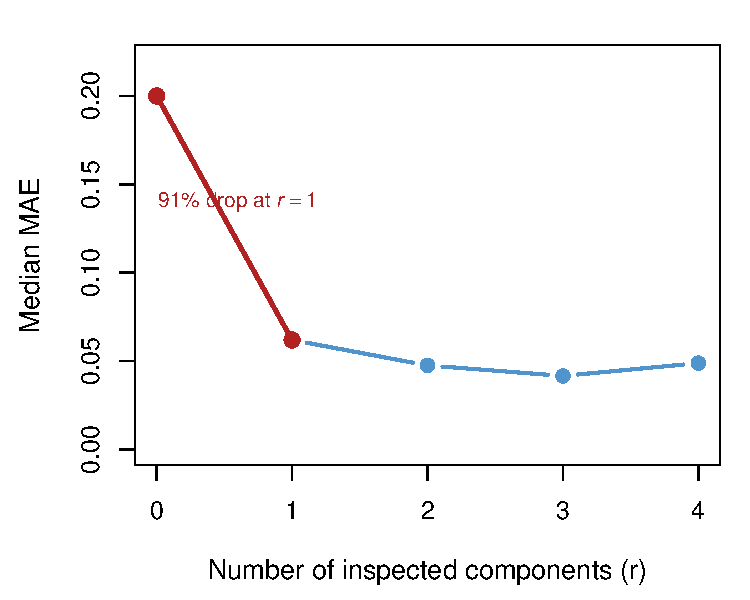
\includegraphics[width=0.65\textwidth]{figures/fig2_autopsy_coverage.pdf}
\caption{Median MAE vs.\ number of inspected components~$r$
  ($m = 4$, $k = 2$, $n = 300$, $R = 50$).  The sharp drop from
  $r = 0$ to $r = 1$ captures 87\% of the total improvement,
  demonstrating the binary identification threshold.}\label{fig:autopsy-coverage}
\end{figure}

The transition from $r = 0$ to $r = 1$ (\cref{tab:autopsy-coverage,fig:autopsy-coverage}) is dramatic: inspecting a
single component) is dramatic: MAE drops from $0.200$ to $0.062$, a
$3.2\times$ improvement that captures 87\% of the total improvement
from $r = 0$ to full autopsy ($r = m$).  Subsequent inspections provide diminishing
returns.  This confirms the phase transition at $r = 1$: the jump is discrete,
not gradual.  The MAE plateaus at $r = 3$ and $r = 4$
($\text{MAE} = 0.042$), indicating that beyond the initial
symmetry-breaking observation, additional inspections yield rapidly
diminishing returns.

\textbf{Interpretation.}  A single inspected component breaks the $m!$
symmetry because knowing whether \emph{one} named component failed or
survived at $\Tsys$ immediately eliminates most of the permutation
equivalences.  With $m = 4$ and $k = 2$, knowing that component~1 failed
reduces the ambiguity from 24 permutations to 6 (only the remaining
$m - 1 = 3$ components can be permuted, and the failed/survived partition
further constrains).  The binary nature of the information---not its
precision---is what matters.

\subsection{Robustness to distributional assumptions}

A Weibull extension ($\alpha = 1.5$, $R = 50$) preserves the ranking:
periodic ($\MAE = 0.053$, $17.0\times$) outperforms masking
($\MAE = 0.099$, $9.0\times$), both far ahead of Scheme~0
($\MAE = 0.887$).  The larger improvement factors reflect the
$2m$-dimensional Weibull parameter space, which amplifies the symmetry
problem.  Additional experiments (variation across $k$, scaling with $m$)
are available in the \texttt{kofn} package vignettes.

% ===========================================================================
% 6. DISCUSSION
% ===========================================================================

\section{Discussion}\label{sec:discussion}

\subsection{Practical recommendations}\label{sec:recommendations}

The experimental results suggest a decision procedure for practitioners:
\begin{enumerate}
  \item \textbf{Can you inspect components during operation?}
    Use periodic inspection.  The temporal resolution is irrelevant
    ($\delta = 2.0$ works as well as $\delta = 0.1$), so even crude
    monitoring suffices.  This is the most effective mechanism overall.

  \item \textbf{Can you inspect any components after system failure?}
    Inspect at least one.  The phase transition at $r = 1$ means that
    even checking a single component's failed/survived status dramatically
    improves estimation.  Each additional inspected component helps, but
    with diminishing returns.

  \item \textbf{Do you know which components failed (perhaps imprecisely)?}
    Use generalized masking.  It is robust to substantial noise
    ($p_{\text{mask}} \leq 0.5$) and adapts naturally to varying
    diagnostic certainty.

  \item \textbf{Do you know the component reliability ordering?}
    This provides essentially no improvement over the baseline.
    Ordering constraints eliminate the mode multiplicity but do not
    sharpen the remaining mode.

  \item \textbf{None of the above.}  Accept the Scheme~0 limitation:
    individual parameters are not identifiable, but the system-level
    parameters (e.g., system failure rate) can still be estimated.
\end{enumerate}

\subsection{Scope and limitations}\label{sec:scope}

\textbf{Series systems ($k = 1$).}
The periodic inspection likelihood \eqref{eq:scheme1-ll} uses a composite
approximation that breaks down for $k = 1$ (see \cref{rem:series-breakdown}).
For series systems, the well-developed masked cause-of-failure literature
\citep{Miyakawa1984, LinUsherGuess1993, CraiuDuchesne2004} provides the
correct framework.  The generalized masking and partial autopsy likelihoods
(\cref{sec:masking,sec:autopsy}) are valid at $k = 1$ and reduce to
standard masked-data formulas.

\textbf{Composite likelihood.}
The periodic inspection likelihood \eqref{eq:scheme1-ll} is a composite
likelihood, not a full joint likelihood.  The full joint would condition
the component intervals on the event that the system failed at $\Tsys$,
which would require integrating over a constrained region of
$\mathbb{R}^m$.  The composite approximation is computationally
tractable and, as our experiments show, highly effective.  However,
standard errors from the observed information may underestimate the
true uncertainty.  A sandwich-type variance correction
\citep{VarinReidFirth2011} could address this, but we leave it for
future work.

\textbf{Computational cost.}
The general system density \eqref{eq:fsys} requires $O(m \cdot 2^{m-1})$
evaluations per time point, making it practical for $m \leq 15$ or so.
For exponential parallel systems, the inclusion-exclusion expansion
(\cref{sec:ie-expansion}) provides $O(2^m)$ closed-form evaluations.
Partial autopsy adds $O(2^{m-r})$ per observation for marginalizing over
uninspected components.

\textbf{Independence assumption.}
Throughout, we assume independent component lifetimes.  Load-sharing
systems \citep{Park2013}, common-cause failures, and dependent degradation
processes would require extensions of both the system density and the
symmetry analysis.

\subsection{Connections to related problems}\label{sec:connections}

\textbf{Label switching in Bayesian mixture models.}
The permutation symmetry in $k$-out-of-$m$ estimation is structurally
identical to the label-switching problem in Bayesian mixture model inference
\citep{Stephens2000, JasraHolmesStephens2005}.  In both settings,
the likelihood is invariant under permutation of component labels, creating
multimodal posteriors.  The Bayesian mixture literature has developed
post-processing techniques (relabeling algorithms, identifiability
constraints) that operate \emph{after} sampling.  Our approach differs:
we break the symmetry \emph{before} estimation by incorporating
component-level data into the likelihood.

\textbf{Identifiability in competing risks.}
For series systems, the non-identifiability of marginal distributions from
the joint survival function is a classical result \citep{Tsiatis1975,
Cox1959}.  \citet{Meilijson1981} showed that autopsy data (observing which
component caused system failure) restores identifiability;
\citet{SarhanElBassiouny2003} developed parallel-system component
estimation under masked data.
\citet{Komarova2017} extended this to $k$-out-of-$m$ systems under
nonparametric assumptions (see also the general incomplete-data framework
of \citealp{DempsterLairdRubin1977}).  Our contribution complements these theoretical
results with a quantitative comparison of the \emph{degree} of identifiability
under different observation mechanisms.

\textbf{Component estimation from system data.}
Several recent papers address the specific problem of estimating component
parameters from system-level observations.
\citet{BhattacharyaSamaniego2010} derived component estimators using
system signatures, while \citet{NgNavarroBalakrishnan2017} and
\citet{YangNgBalakrishnan2019} developed stochastic EM algorithms for
system lifetime data with known and unknown signatures, respectively.
\citet{DembinskaJasinski2021} studied MLE from discrete $k$-out-of-$n$
component lifetimes.  \citet{RodriguesPereira2019} considered masked
data in general coherent systems.  Our work complements these by
systematically comparing the \emph{type} of supplementary information
needed rather than developing estimators for a single observation scheme.

\textbf{Optimal experimental design.}
Our sensitivity results---especially the $\delta$-insensitivity and the
$r = 1$ phase transition---have implications for experimental design in
reliability testing.  Given a budget for component monitoring,
the results suggest investing in \emph{breadth} (inspecting more systems
with minimal monitoring) rather than \emph{depth} (fine-grained monitoring
of fewer systems).  This connects to optimal design theory for reliability
experiments \citep{AtkinsonDonev1992}, which typically focuses on sample
size and censoring time allocation, not monitoring granularity.

% ===========================================================================
% 7. SOFTWARE
% ===========================================================================

\section{Software}\label{sec:software}

All methods described in this paper are implemented in the open-source R
package \texttt{kofn}, available at
\url{https://github.com/queelius/kofn} and via
\href{https://queelius.r-universe.dev}{r-universe}.
The package name follows the conventional ``$k$-out-of-$n$'' terminology;
this paper uses $m$ for the number of components to avoid collision with
sample size~$n$.

\textbf{Architecture.}
The package provides a single constructor \texttt{kofn(k, m, family)}
that returns an S3 object inheriting from the \texttt{likelihood\_model}
class.  Generic methods \texttt{loglik()}, \texttt{score()},
\texttt{hess\_loglik()}, and \texttt{fit()} follow the closure-returning
convention: \texttt{loglik(model)} returns a function
\texttt{function(df, par)} that evaluates the log-likelihood at
parameters \texttt{par} given data \texttt{df}.

\textbf{Key functions.}
\begin{itemize}
  \item \texttt{loglik\_scheme1()}, \texttt{fit\_scheme1()},
    \texttt{rdata\_scheme1()}: Periodic inspection (Scheme~1).
  \item \texttt{loglik\_masked()}, \texttt{rdata\_masked()}: Generalized
    masking for arbitrary $k$.
  \item \texttt{observe\_right\_censor()}, \texttt{observe\_periodic()},
    \texttt{observe\_exact()}: Composable observation functors.
  \item \texttt{coherent\_system()}, \texttt{kofn\_system()}: System
    infrastructure with precomputed critical states.
  \item \texttt{ie\_expand()}: Inclusion-exclusion expansion for
    exponential parallel systems.
\end{itemize}

\textbf{Quality.}
The package has 307 \texttt{testthat} tests with 93\% line coverage and
passes \texttt{R CMD check} cleanly.  The Monte Carlo experiments in this
paper are reproducible via precomputed results stored in
\texttt{inst/precomputed/paper/}.

\textbf{Ecosystem.}
The package connects to the reliability ecosystem described in
\citet{MeekerEscobarPascual2022}: it uses the
\texttt{likelihood.model} package for the \texttt{fisher\_mle} result class
(providing \texttt{coef()}, \texttt{vcov()}, \texttt{logLik()},
\texttt{AIC()}, \texttt{confint()}, \texttt{summary()}) and
\texttt{numDeriv} \citep{numDeriv} for numerical derivatives.

% ===========================================================================
% 8. CONCLUSION
% ===========================================================================

\section{Conclusion}\label{sec:conclusion}

We have shown that estimating individual component parameters from
$k$-out-of-$m$ system data is fundamentally limited by permutation
symmetry in the system density, and that breaking this symmetry requires
component-level information.  Three mechanisms---periodic inspection,
generalized masking, and partial autopsy---provide $3.5$--$7.0\times$
improvement over system-only data, while domain knowledge (ordering
constraints, heterogeneous fleet data) provides negligible help.

Two findings deserve particular emphasis.  First, the phase transition at
$r = 1$: inspecting a single component captures most of the benefit of
full autopsy.  For practitioners, this means that even minimal post-failure
diagnosis---checking whether one specific component failed---is far more
valuable than sophisticated statistical machinery applied to system-level
data alone.  Second, the complete insensitivity to temporal resolution:
the binary fact of \emph{which} component failed matters infinitely more
than the precision of \emph{when}.  Coarse monitoring ($\delta = 2.0$)
works as well as fine monitoring ($\delta = 0.1$).

Several directions remain open.  The composite likelihood for periodic
inspection could be replaced with a full conditional likelihood, at the
cost of integration over constrained regions.  Optimal inspection design
(which $r$ components to inspect, given a budget) connects to experimental
design theory.  Extensions to dependent component lifetimes and degradation
models would broaden the practical applicability.  Finally, a Bayesian
treatment with informative priors on the component ordering could combine
the strengths of domain knowledge and component-level data.

% ===========================================================================
% ACKNOWLEDGMENTS
% ===========================================================================

\section*{Acknowledgments}

Computations were performed in R \citep{RCore2025}.

% ===========================================================================
% APPENDICES
% ===========================================================================

\appendix

\section{Proof of \texorpdfstring{\cref{prop:symmetry}}{Proposition 1}}
\label{sec:proof-symmetry}

We provide the full proof of the permutation invariance of the system
density for $k$-out-of-$m$ systems.

\begin{proof}
Let $\pi$ be a permutation of $\{1, \ldots, m\}$.  Define
$\blambda_\pi = (\lambda_{\pi(1)}, \ldots, \lambda_{\pi(m)})$.  Under
the permuted parameters, component $j$ has rate $\lambda_{\pi(j)}$.
The system density under $\blambda_\pi$ is
\begin{equation}\label{eq:proof-step1}
  \fsys(t; \blambda_\pi) = \sum_{j=1}^{m} f_j(t; \lambda_{\pi(j)})
    \sum_{\substack{\bx_{-j}: j \text{ critical}}}
    \prod_{\ell \neq j} p_\ell(x_\ell, t; \lambda_{\pi(\ell)}).
\end{equation}

For a $k$-out-of-$m$ system, the critical states for component $j$ depend
only on the \emph{number} of other components that have failed, not on
their identities: component $j$ is critical precisely when $k - 1$ of the
remaining $m - 1$ components have failed.  The set of critical state
vectors $\bx_{-j}$ is therefore the set of all binary vectors of length
$m - 1$ with exactly $k - 1$ ones.

Now substitute $\ell' = \pi^{-1}(\ell)$ in the outer sum and rearrange
the inner products.  Since the collection of all $(k-1)$-subsets of
$\{1, \ldots, m\} \setminus \{j\}$ is mapped bijectively to the
collection of all $(k-1)$-subsets of $\{1, \ldots, m\} \setminus
\{\pi^{-1}(j)\}$ under $\pi^{-1}$, and since each product term depends
only on the rate assigned to that component (not the component label),
the sum \eqref{eq:proof-step1} is a rearrangement of the sum in
\eqref{eq:fsys} evaluated at $\blambda$.

Concretely, letting $j' = \pi^{-1}(j)$:
\[
  \fsys(t; \blambda_\pi)
  = \sum_{j'=1}^{m} f_{j'}(t; \lambda_{j'})
    \sum_{\substack{\bx_{-j'}: j' \text{ critical}}}
    \prod_{\ell' \neq j'} p_{\ell'}(x_{\ell'}, t; \lambda_{\ell'})
  = \fsys(t; \blambda).
\]
The first equality uses the fact that the substitution $j = \pi(j')$ is a
bijection on $\{1, \ldots, m\}$ and that the critical states for
$\pi(j')$ under $\blambda_\pi$ correspond to the critical states for
$j'$ under $\blambda$.  The second equality is the definition
\eqref{eq:fsys}.
\end{proof}

\section{Inclusion-Exclusion Expansion}
\label{sec:ie-expansion}

For exponential parallel systems ($k = m$), the product $\prod_{i \neq j}
(1 - e^{-\lambda_i t})$ can be expanded via inclusion-exclusion:
\begin{equation}\label{eq:ie}
  \prod_{i \neq j} (1 - e^{-\lambda_i t})
  = \sum_{S \subseteq \{1,\ldots,m\} \setminus \{j\}}
    (-1)^{|S|} \exp\Bigl(-\sum_{i \in S} \lambda_i \cdot t\Bigr).
\end{equation}
This has $2^{m-1}$ terms, each a pure exponential in $t$.  The component
contribution $w_j(t) = \lambda_j e^{-\lambda_j t} \prod_{i \neq j}
(1 - e^{-\lambda_i t})$ is therefore a signed sum of $2^{m-1}$
exponentials:
\[
  w_j(t) = \lambda_j \sum_{S \subseteq \{1,\ldots,m\} \setminus \{j\}}
    (-1)^{|S|} \exp\bigl(-(\lambda_j + \textstyle\sum_{i \in S} \lambda_i)
    \cdot t\bigr).
\]

This representation makes all integrals closed-form:
\[
  \int_a^b w_j(t)\, dt = \lambda_j
    \sum_S (-1)^{|S|} \frac{e^{-r_S a} - e^{-r_S b}}{r_S},
\]
where $r_S = \lambda_j + \sum_{i \in S} \lambda_i$.  This is used for
interval-censored and left-censored observations in the Scheme~0 and
Scheme~1 likelihoods.  The expansion has $O(2^m)$ terms and is practical
for $m \leq 15$.

\section{Partial Autopsy Enumeration}
\label{sec:autopsy-algorithm}

\begin{algorithm}[t]
\caption{Partial autopsy likelihood evaluation for one observation.}
\label{alg:autopsy}
\begin{algorithmic}[1]
\Require{System time $t$, inspected set $\mathcal{I}$, observed failed
  set $F_{\text{obs}}$, observed survived set $S_{\text{obs}}$,
  parameters $\btheta$, system parameter $k$}
\State $\mathcal{U} \gets \{1,\ldots,m\} \setminus \mathcal{I}$
  \Comment{uninspected components}
\State $k_{\text{unk}} \gets k - |F_{\text{obs}}|$
  \Comment{failures needed from uninspected}
\If{$k_{\text{unk}} < 0$ \textbf{or} $k_{\text{unk}} > |\mathcal{U}|$}
  \State \Return $-\infty$ \Comment{inconsistent observation}
\EndIf
\State $L \gets 0$
\For{each $U \in \binom{\mathcal{U}}{k_\text{unk}}$}
  \Comment{enumerate unknown failed subsets}
  \State $F \gets F_{\text{obs}} \cup U$
  \Comment{full failed set}
  \For{each $j \in F$}
    \Comment{critical component}
    \State $\text{term} \gets f_j(t) \cdot
      \prod_{\ell \in F \setminus \{j\}} F_\ell(t) \cdot
      \prod_{\ell \notin F} S_\ell(t)$
    \State $L \gets L + \text{term}$
  \EndFor
\EndFor
\State \Return $\log L$
\end{algorithmic}
\end{algorithm}

\Cref{alg:autopsy} gives the pseudocode for evaluating the partial
autopsy likelihood \eqref{eq:autopsy-ll} for a single observation.  The
outer loop enumerates all $\binom{m-r}{k_{\text{unk}}}$ possible
assignments of the unknown failures to uninspected components.  The inner
loop over $j \in F$ computes the system density contribution for each
candidate critical component.  Total cost per observation is
$O(\binom{m-r}{k_{\text{unk}}} \cdot k)$.

% ===========================================================================
% BIBLIOGRAPHY
% ===========================================================================

\bibliographystyle{plainnat}
\bibliography{paper}

\end{document}
